\documentclass[10pt]{article}
\usepackage[utf8]{inputenc}
\usepackage[T1]{fontenc}
\usepackage{graphicx}
\usepackage{appendix}
\usepackage[french]{babel}
\usepackage{fancyhdr}
\usepackage{geometry}
\geometry{hmargin=3cm,vmargin=3.5cm}
\usepackage{enumitem}
\usepackage{listings}
\usepackage{subcaption}
\usepackage{amsmath}
\usepackage{animate}
\graphicspath{{./img/}}
\lstset{ %
  backgroundcolor=\color{white},   % choose the background color; you must add \usepackage{color} or \usepackage{xcolor}
  basicstyle=\small,               % the size of the fonts that are used for the code
  breakatwhitespace=false,         % sets if automatic breaks should only happen at whitespace
  breaklines=true,                 % sets automatic line breaking
  captionpos=b,                    % sets the caption-position to bottom
  commentstyle=\color{blue},      % comment style
%  escapeinside={\%*}{*)},          % if you want to add LaTeX within your code
  extendedchars=true,              % lets you use non-ASCII characters; for 8-bits encodings only, does not work with UTF-8
  frame=single,                    % adds a frame around the code
  keepspaces=true,                 % keeps spaces in text, useful for keeping indentation of code (possibly needs columns=flexible)
%  keywordstyle=\color{blue},       % keyword style
  language=C,                    % the language of the code
  numbers=left,                    % where to put the line-numbers; possible values are (none, left, right)
  numbersep=5pt,                   % how far the line-numbers are from the code
  numberstyle=\tiny\color{black},  % the style that is used for the line-numbers
  rulecolor=\color{black},         % if not set, the frame-color may be changed on line-breaks within not-black text (e.g. comments (green here))
  showspaces=false,                % show spaces everywhere adding particular underscores; it overrides 'showstringspaces'
  showstringspaces=false,          % underline spaces within strings only
  showtabs=false,                  % show tabs within strings adding particular underscores
  stepnumber=1,                    % the step between two line-numbers. If it's 1, each line will be numbered
  tabsize=2,                       % sets default tabsize to 2 spaces
}
\usepackage{hyperref}
\usepackage{minted}
\hypersetup{colorlinks=true}

\pagestyle{fancy}

\renewcommand{\sectionmark}[1]{ \markright{#1}{} }

\lhead{}
\rhead{}
\lfoot{ENSEIRB-MATMECA}
\rfoot{PRCD}
\renewcommand{\headrulewidth}{0.pt}
\renewcommand{\footrulewidth}{0.4pt}


\title{TDP1}
\author{Arnaud Durocher, Alexandre Honorat}
\date{\today}

\begin{document}
%\tableofcontents
%\newpage

\thispagestyle{empty}


%\begin{center}
%
\includegraphics{enseirb_inp.png}
%\end{center}
%
%\vspace{\stretch{1}}
\hrule
\begin{flushleft}
\Huge{\textbf{TDP4 - Utilisation de MPI}}\\
\textit{Lancer de Rayons}
\end{flushleft}
\begin{flushright}
\huge\textbf{Rapport}\\
\end{flushright}
\hrule

\vspace{80pt}
\noindent\textbf{Élèves :}
\emph{Alexandre Honorat}, \emph{Elouan Keryell-Even}\\
\\
\noindent\textbf{Responsable :}
\emph{Astrid Casadei}\\


\vspace{60pt}
\normalsize
\begin{center}
  Troisième année, filière informatique, option PRCD\\
  Date : \today\\
  Enseirb-Matmeca
\end{center}
\vspace{50pt}

%% -*- eval: (flyspell-mode 1); -*-

\chapter{Introduction}
%\addcontentsline{toc}{chapter}{Introduction}

Un des aspects de la recherche informatique consiste à améliorer des programmes afin de rendre leur temps d'exécution plus rapide, il s'agit du \emph{calcul haute performance} (ou HPC, pour High Performance Computing). 
%Les performances -- en matière de temps d'exécution -- sont primordiales par exemple pour les codes de simulation numérique dédiés à la météorologie qui calculent les prévisions du lendemain, où bien entendu la simulation doit donc s'être terminée en moins d'une nuit. 
Dans ce cadre le stage a porté sur la génération automatique de certains de ces programmes améliorés. 
Les sections suivantes présentent brièvement quelques rappels sur les problématiques HPC, ainsi que l'objectif du stage : l'adaptation automatique d'une certaine catégorie de problèmes au matériel prévu pour le HPC. Le chapitre $2$ précise plus particulièrement ces problématiques et l'objectif tandis que le chapitre $3$ se concentre sur le travail réalisé. Le chapitre $4$ en propose une évaluation et est suivi par la conclusion. 


\section{Parallélisation de programmes}

Diverses techniques existent pour améliorer les performances d'un programme et plus particulièrement de son temps d'exécution. Deux aspects peuvent entrer en compte : les algorithmes utilisés dans le programme ainsi que le matériel qui l'exécute. Le facteur limitant à améliorer en priorité est alors le matériel, car il influe sur la nature des algorithmes pouvant être utilisés.

La solution la plus simple pour améliorer les performances consisterait à se baser uniquement sur la loi de Moore, c'est-à-dire sur le fait que les capacités du matériel sur lequel le programme est exécuté sont doublées tous les ans. Or cette loi exponentielle n'est maintenant plus valable puisque la fréquence d'horloge des processeurs modernes stagne depuis quelques années à une valeur proche de $3$ GHz. 
%C'est cette fréquence d'horloge qui impose au matériel (si celui-ci est constitué de cet unique processeur) le nombre d'opérations qu'il va pouvoir effectuer en une seconde. Puisque la fréquence n'augmente plus, le nombre d'opérations par seconde pour ce type de matériel ne peut plus augmenter non plus, aucun gain de rapidité d'exécution n'est alors possible.

%La première solution s'appuyait ainsi sur l'augmentation de la fréquence, c'est-à-dire de la rapidité de chaque opération sachant qu'une seule est faite à la fois. Au lieu d'augmenter la rapidité des opérations, 
Une solution est d'augmenter le nombre d'opérations effectuées \emph{en même temps} par un processeur, ce qui est l'introduction du parallélisme dans le matériel.
%Celui-ci peut s'effectuer de plusieurs manières : à l'intérieur et à l'extérieur du processeur. À l'intérieur,
Il s'agit soit de subdiviser les instructions en  micro-instructions afin de créer un pipeline (ainsi une instruction peut commencer immédiatement après la fin de la première micro-instruction de l'instruction précédente), soit de dupliquer certains composants de l'architecture afin d'exécuter plusieurs instructions sur à la fois, soit enfin l'application de la même instruction sur plusieurs données à la fois. Les processeurs modernes intègrent tous ces trois technologies : le pipeline d'instructions, l'architecture nommée \emph{superscalaire}, et les calculs dits \emph{vectoriels}.
%À l'extérieur il s'agit de connecter plusieurs processeurs les uns avec les autres, tous participant aux calculs nécessités par le programme de base. Différentes manières de relier les processeurs existent, ils peuvent alors être appelés des cœurs ; dans toute la suite du rapport, un processeur est synonyme d'un ensemble de cœurs connectés entre eux par de la mémoire cache hiérarchique en accès uniforme\footnote{Cette notion sera explicitée au point \ref{sec:stencil_base}.}.
Les processeurs peuvent eux-mêmes être répliqués dans leur ensemble, soit sur une même surface de silicium (processeurs multicœurs), soit distinctement et alors reliés par un bus (multiprocesseurs), soit encore par une combinaison de ces deux techniques.
Enfin en dehors des processeurs classiques -- ou \emph{centraux}, abrégés en CPU -- existent aussi des processeurs graphiques -- dénommés GPU --, qui contiennent beaucoup de cœurs mais exécutent obligatoirement tous la même instruction en même temps. Bien sûr les deux types peuvent coexister sur une même machine.

La nature du matériel (et non seulement ses capacités d'ordre physique comme la fréquence d'horloge) nécessite une conception des algorithmes en adéquation (par exemple pour utiliser le côté superscalaire). 
%cela induit des modifications dans la façon de transcrire les algorithmes (par exemple pour utiliser le côté superscalaire), ainsi que dans les algorithmes eux-mêmes qui ne sont parfois plus du tout adaptés (notamment à cause des communications entre les processeurs, inexistantes auparavant). 
Écrire un programme destiné à une machine parallèle impose donc d'avoir des algorithmes souvent très spécifiques à la configuration de la machine d'exécution, ce qui est d'autant plus complexe avec les architectures des machines actuelles de plus en plus hétérogènes, et peut poser des problèmes de portabilité des applications.

\section{\'Ecriture de code parallèle}

%Les algorithmes étant souvent spécifiques au type de parallélisme et à l'architecture de la machine cible, les langages permettant d'écrire des programmes parallèles automatisent difficilement la génération de codes parfaitement adaptés à la machine cible. En pratique la plupart des langages modernes permettent l'expression du parallélisme sans le découvrir eux-même ; certains outils aident à écrire du code parallèle mais ils sont souvent expérimentaux et nécessitent alors que le code automatiquement produit soit vérifié avant d'être compilé\footnote{Lors de la transcription d'un problème en informatique, il est d'abord nécessaire de transcrire le problème vers un langage informatique (le code) -- compréhensible par les humains -- qui est alors \emph{compilé} par un programme préexistant (le compilateur) qui le transforme en fichier binaire exécutable -- compréhensible par \emph{la} machine.}.

Le procédé classique consiste à premièrement décrire le problème de manière algorithmique, deuxièmement à le transcrire dans un langage de programmation donnée -- et utiliser les outils natifs du langage ou alors les bibliothèques spécifiques pour le parallélisme -- et troisièmement à compiler le code écrit à l'étape précédente grâce à différents outils internes au compilateur. Les deux premières étapes sont réalisées par le développeur, à qui il convient de faciliter la tâche. 

Les difficultés inhérentes à la production d'un programme parallèle sont de plusieurs natures, notamment l'identification des sections parallèles et de celles obligatoirement séquentielles, ainsi que la gestion des communication et l'utilisation de toutes les ressources disponibles sur la matériel. L'identification des régions parallélisables ou non dépend de l'algorithme utilisé pour résoudre le problème voulu. Un programme bien parallélisé réduit au maximum le nombre d'opérations qui sont exécutées séquentiellement, afin que la majeure partie du temps d'exécution soit passée dans des sections parallèles où toute la puissance de la machine parallèle est utilisée. Par ailleurs il est essentiel de gérer les communications entre les différents processeurs afin que des calculs puissent être effectués pendant les communications ; on parle alors du recouvrement des communications. Enfin il convient d'utiliser le plus de ressources possibles sans que cette utilisation n'entraîne d'effort trop important, par exemple si de nombreuses parties de l'algorithme nécessitent une synchronisation de tous les processeurs -- ce qui est très coûteux en temps.

Actuellement c'est au programmeur qu'incombent presque toutes les tâches de parallélisation\footnote{En ce qui concerne les capacités des compilateurs, \textsf{gcc} comprend les directives de la bibliothèque \textsf{OpenMP}, mais ne les trouve pas automatiquement (bien qu'elles soient souvent très simples) et c'est donc au programmeur de les écrire. En revanche les compilateurs modernes sont capables d'exploiter eux-mêmes la caractère superscalaire d'un processeur, mais pas toujours de manière optimale. De même certains calculs vectoriels peuvent être détectés automatiquement, mais ils sont le plus souvent déclenchés via des fonctions spécifiques appelées par le développeur.}. %, or cela nécessite beaucoup de compétences, de temps, et de tests avant de parvenir à un résultat acceptable. S'il n'est pas toujours possible de découvrir le parallélisme automatiquement, il n'est pas non plus toujours facile de savoir où le décrire. Alors que 
Certaines options sont très proches du processeur (comme les capacités vectorielles) et doivent être gérées de manière assez fines, d'autres peuvent être prises en charge à un plus haut-niveau comme le lancement de plusieurs procédures distinctes en parallèle (a priori chacune des procédures étant alors associée à un processeur libre). %Cela amène à une hiérarchisation du parallélisme, ce qui complique encore plus la tâche du programmeur.
Par ailleurs certains paramètres du programme peuvent êtres calculés lors de la compilation -- paramètres statiques -- et d'autres uniquement lors de l'exécution -- paramètres dynamiques. Or pour améliorer la rapidité du programme, il est souhaitable de limiter les calculs lors de l'exécution. Lorsque le programmeur écrit un code en HPC, il espère donc avoir le plus possible de paramètres statiques, selon les possibilités du compilateur et du langage. 

Une des problématiques du parallélisme est donc de faciliter l'écriture de programme, soit en découvrant automatiquement le parallélisme -- ce qui est plutôt difficile -- , soit en fournissant au programmeur des outils adaptés -- ce qui est un peu plus facile.

\section{Choix du niveau d'expression du parallélisme}

%Pour écrire un programme informatique résolvant un problème donné, il est nécessaire de passer par de nombreuses étapes intermédiaires qui sont tout autant de stades où le parallélisme peut être décrit. De très nombreuses possibilités existent et nous ne les présenteront pas en intégralité ici. 

Compte-tenu de la complexité de l'écriture de code parallèle, des outils spécifiques ont été mis en place afin de faciliter le développement de tels programmes. Or ces outils -- langages, bibliothèques, ou compilateur -- sont rares et souvent trop spécifiques ou au contraire trop généraux. L'objectif du stage est donc de développer un nouvel outil adapté à un certain type de problèmes pour lequel peu d'outils existent et ne sont pas adaptés à la configuration hétérogène des machines actuelles.

Introduire un nouveau langage dédié au parallélisme est complexe car il faut non seulement développer le compilateur et les bibliothèques standards associés , mais aussi le rendre simple à utiliser et si possible pas trop éloigné des autres paradigmes dominants afin de faciliter son appréhension. D'un autre côté garder les langages existants implique de modifier les compilateurs pour qu'ils découvrent automatiquement les possibilités de parallélisation, ce qui est difficile à mettre en œuvre -- à cause de la complexité même de trouver le parallélisme, et à cause de la complexité des compilateurs modernes.
%Les deux solutions existent actuellement avec un succès mitigé\footnote{Ce constat est difficile à vérifier, mais à titre d'exemple les langages intrinsèquement parallèles que sont \textsf{Chapel} ou \textsf{Cilk} voire \textsf{Erlang} ne sont pas enseignés dans la filière PRCD de l'Enseirb-Matmeca, probablement car ils ne sont pas suffisamment répandus. Par ailleurs pour les capacités des compilateurs, \textsf{gcc} comprend les directives de la bibliothèque \textsf{OpenMP}, mais ne les trouve pas automatiquement (bien qu'elles soient souvent très simples), en revanche les compilateurs modernes sont souvent capables d'exploiter eux-mêmes la caractère superscalaire d'un processeur.}.

%Dans le cadre du stage, nous nous sommes alors plutôt intéressés aux possibilités d'un Domain Specific Embedded Language (DSEL, équivalent de \emph{langage spécifique embarqué} en français) qui permet une charge de développement moindre, ainsi qu'une appréhension rapide. En effet il s'agit alors d'une bibliothèque fournie au programmeur dans un langage courant préexistant, ne comportant que quelques fonctions reprenant uniquement les paradigmes dont le programmeur a besoin pour résoudre un type de problème spécifique, et se basant sur des bibliothèques performantes préexistantes. 
Nous avons donc décidé de développer une approche basée sur un Domain Specific Embedded Language (DSEL, équivalent de \emph{langage spécifique embarqué} en français) sous la forme d'une bibliothèque, avec comme objectifs de faciliter la prise en main du programmeur et de réduire sa charge de développement, tout en préservant ou en améliorant les performances de ses programmes.
% à recaser plus tard
%Le DSEL se différencie d'un DSL (équivalent de \emph{langage spécifique}) par le fait qu'il est disponible au sein d'un langage général, et permet donc potentiellement au développeur d'effectuer des tâches connexes à la résolution du problème dans un seul et même langage. Il peut ainsi utiliser plusieurs DSEL dans le même code, et donc résoudre des problèmes complexes avec un formalisme adapté à chacun d'entre eux (et par là-même avoir de meilleures performances). Le DSEL est ainsi une solution intermédiaire efficace, qui nous a semblé adaptée à l'objectif du stage qui est la parallélisation automatique d'une catégorie spécifique de programmes. 
Plutôt que de focaliser ce DSEL sur un type spécifique de parallélisme, ou sur un paradigme comme le font de nombreux outils, ce DSEL est focalisé sur une catégorie de problèmes et doit permettre de cacher justement tout ce qui relève du parallélisme.




\section{Version minimale}

Dans un premier lieu, nous avons décidé de commencer par faire une version minimale du simulateur de particules. Cette première version modélise les particules, applique les formules pour les mettre à jour en utilisant des communications ni persistantes, ni recouvertes par le calcul et avec un \textbf{dt} constant.

Dans cette partie, nous verrons comment les particules ont été modélisées et comment leurs valeurs sont mises à jour entre chaque itération.

\subsection{Principe de mise à jour des particules}

Le but est d'appliquer les formules de l'équation (\ref{eq:modele_physique}) vue dans l'introduction, sur toutes les particules distribuées dans les différents processus. Chacun des $p$ processus possède en mémoire locale $n$ particules.

Chaque processus est chargé de mettre à jour l'état de ses particules locales, et doit pour chacune de celles-ci calculer les forces induites par toutes les autres particules, y compris celles des autres processus. Afin de connaître les informations sur toutes les particules, les processus communiquent entre eux avec une topologie en forme d'anneau.

Chaque processus reçoit de son voisin un paquet de particule et accumule les forces induites par le paquet reçu, jusqu'à avoir parcouru tous les paquets. En supposant qu'il y ait $p$ processus contenant $n$ particules, la somme est découpée de la façon suivante:

\begin{equation}
      \overrightarrow{a_i} = \sum_{k=0}^{p-1}{\sum_{j=0}^{n-1}{F(p_i^0,p_j^k)}} 
\label{eq:accel_paquets}
\end{equation}
avec $p_i^k$ la $i^{eme}$ particule du processus $k$. Le processus courant prote le numéro $0$.

Entre chaque élément de la première somme, chaque processus reçoit un nouveau paquet de particules qui écrase un ancien paquet pour garder le caractère distribué des données.

\paragraph{Complexité du calcul}

Chaque processeur doit calculer les forces entre ses particules locales et toutes les autres. La complexité du calcul est en $\theta(pn^2)$ par itération. En terme de communications, chaque processus envoie et reçoit $p$ messages de taille $n$.

Le caractère quadratique des calculs et la taille linéaire des messages font que les communications sont recouvrables par le calcul pour peu que $n$ soit suffisamment grand.

\subsection{Modélisation des particules}

Les particules sont représentées de deux manières différentes selon qu'il s'agisse des particules locales ou distantes. On se place ici toujours en dimension 2.

La force ne dépend que de la position de de la masse de la particule distante, donc ces données suffisent à les modéliser. La structure modélisant les particules distante est alors la suivante:
\begin{minted}{c}
struct mpi_particle {
  double px, py;
  double mass;
};
\end{minted}
Cette structure est celle utilisée lors des communications, il a donc fallu créer un type MPI qui lui est associé avec \texttt{MPI\_Type\_create\_struct} que nous avons nommé \texttt{MPI\_Type\_particles}.

Les particules locales possèdent en revanche d'autres propriétés comme la vitesse et l'accélération:
\begin{minted}{c}
struct particle {
  double px, py;
  double vx, vy;
  double ax, ay;
  double mass;
};
\end{minted}

\subsection{Communications}

Dans cette première version, les communications se font de manière non persistante et ne sont pas recouvertes par du calcul. Chaque processus reçoit du processus précédent et envoie vers le processus suivant.

Les communications sont faites de la manière suivante:
\begin{minted}{c}
for(i=0; i<nb_proc-1; i++){
    MPI_Isend(particles_current, [...], rank+1, [...], &send_request);
    MPI_Irecv(particles_next, [...], rank-1, [...], &recv_request);
    MPI_Request requests[] = {send_request, recv_request};
    MPI_Waitall(2, requests, [...]);
    
    [Calcul sur particles_current]
    
    SWAP(particles_current, particles_next);
}
\end{minted}
Le double buffering est effectué sur les buffers \texttt{particles\_current} et \texttt{particles\_next} qui sont échangés à chaque tour de boucle. \texttt{particles\_current} est le buffer contenant le paquet de particules qui induisent les forces calculées à ce tour de boucle, alors que \texttt{particles\_next} est le paquet suivant qui a déjà été reçu.

Les communications asynchrones permettent d'envoyer et de recevoir en même temps et ainsi de gagner du temps par rapport à des communications synchrones. Avec des communications asynchrones, il est déjà possible de recouvrir par le calcul en plaçant ce dernier avant le \texttt{MPI\_Waitall} mais il faut alors faire attention de ne pas modifier le buffer d'envoi.




\subsection{Visualisation et benchmark}

Un travail à été fait pour permettre d'exécuter la simulation sur plusieurs itérations et de visualiser le résultat. Des outils de benchmark ont aussi été mis en place.

Des paramètres d'exécutions permettent de modifier plusieurs paramètres, tels que l'utilisation d'un fichier d'entrée, la génération ou non de données de visualisation, etc...

\subsubsection{Visualisation}

La visualisation se fait à l'aide d'un script GNUPlot. Le programme génère un fichier de données et le script affiche ces données sous la forme d'une image GIF animée. Les particules sont représentées par des cercles dont le rayon représente la masse de la particule.

Lors de la génération des données, une image est générée à intervalle constant (en temps de simulation), même avec un dt variable. En accordant la fréquence de rafraîchissement du GIF dans le script GNUPlot à cet intervalle, nous voyons le déroulement de la simulation à vitesse normale

\subsubsection{Benchmark}

Le temps de calcul total est relevé avec \texttt{gettimeofday} afin de mesurer les performances du simulateur. Différents scripts permettent de générer automatiquement des graphiques des performances.

\section{Améliorations et optimisations}

Différentes améliorations étaient proposées dans le sujet pour augmenter les performances et la précision de la simulation. Nous avons mis en place des communications persistantes, et utilisé un \textbf{dt} variable.

\subsection{Optimisation des communications}

La version de base utilisait déjà des communications asynchrones pour envoyer et recevoir des données en même temps, mais l'envoi n'était pas recouvert par du calcul et la connexion était réinitialisée à chaque envoi. Utiliser les communications persistantes nous a permis d'économiser les temps de connexion à chaque transfert en gardant toujours le canal ouvert. La seconde optimisation que nous avons effectué est le recouvrement des communications par le calcul qui permet de rendre les communications transparentes en remplaçant les temps d'attente par du calcul.

\subsubsection{Communications persistantes}

Les communications persistantes permettent de maintenir un canal de communication ouvert afin de ne pas avoir à ré-établir la connexion à chaque envoi. De telles communications s'initialisent avec les fonctions \texttt{MPI\_Send/Recv\_init} qui associent définitivement une connexion représentée par un \texttt{MPI\_Request} et un buffer de réception/envoi. Il suffit alors de remplacer les appels à \texttt{MPI\_Isend/recv} par un appel à \texttt{MPI\_Start} sur la bonne connexion.

Le double buffering pose cependant un problème. Les buffers d'envoi et de réception sont échangés entre 2 tour de boucles, il faut donc utiliser des connexions différentes. C'est pourquoi il nous a fallu ouvrir 4 connexions pour envoyer et recevoir dans chaque buffer. On échange les buffers de réception et d'envoi en choisissant les bonnes connexion

Le code gérant les communications se présente sous la forme présentée en figure \ref{algo:persist}
\begin{figure}
\begin{minted}{c}
[Allocation de b1 et b2]
MPI_Request send_b1, send_b2, recv_b1, recv_b2;
MPI_Send_init(b1, [...], rank+1, [...], &send_b1);
MPI_Send_init(b2, [...], rank+1, [...], &send_b2);
MPI_Recv_init(b1, [...], rank-1, [...], &recv_b1);
MPI_Recv_init(b2, [...], rank-1, [...], &recv_b2);
[Initialisation de b1 avec les particules locales]
for(i=0; i<nb_proc-1; i++){
    MPI_Request* recv, send;
    if(i%2){
        send = &send_b1;
        recv = &recv_b2;
        particles_current = b1;
    } else {
        send = &send_b2;
        recv = &recv_b1;
        particles_current = b2;
    }
    MPI_Start(send_request);
    MPI_Start(recv_request);
    [Calcul sur particles_current]
    MPI_Request requests[] = {*send_request, *recv_request};
    MPI_Waitall(2, requests, [...]);
}
\end{minted}
\caption{Communications persistantes}
\label{algo:persist}
\end{figure}

\subsubsection{Recouvrement des communications}

Le recouvrement de données consiste à effectuer des calculs pendant les communications. Placer les calculs entre \texttt{MPI\_Start} et \texttt{MPI\_Waitall} permet de les effectuer sans attendre que la communication ne termine. Pour que cela fonctionne, il faut s'assurer que les buffers d'envoi et de réception ne soient pas modifiés. Ici, il est possible d'accéder au buffer d'envoi en lecture seule, dans la mesure où les particules distantes ne sont pas modifiées lors du calcul de la force.

Le recouvrement des communications par du calcul devrait compenser le temps de latence de la communication.


\subsection{\textbf{dt} variable}

Avec la discrétisation, l'accélération est considérée constante sur la durée dt, ce qui mène à des erreurs d'approximation. Les erreurs sont d'autant plus importantes que dt est grand, que les particules sont proches et que la vitesse est importante.

On souhaite avoir $dt$ tel que pour toute particule i $\|\delta \overrightarrow{p_i}\| < 0.1 \|\overrightarrow{p_i} - \overrightarrow{p_j}\|$ avec j la particule la plus proche de i. On approxime l'inéquation avec l'inégalité triangulaire et on cherche dt tel que $\|\overrightarrow{v_i}\|dt + |\overrightarrow{a_i}\|\frac{dt^2}{2} = 0.1 \|\overrightarrow{p_i} - \overrightarrow{p_j}\|$. On peut trouver $\|\overrightarrow{p_i} - \overrightarrow{p_j}\|$ lors du calcul de la force où l'on calcule déjà cette valeur. On résout ensuite l'équation du second degré en dt et on trouve un dt par particule. Le $dt$ à choisir est le minimum des $dt$ calculés pour chaque particule. On fait un minimum local au processus, puis une réduction pour trouver le minimum de tous les processus.

A posteriori, la valeur de 0.1 nous a semblé encore trop grande dans la mesure ou certaines particules se comportant encore de façon étrange et semblaient ne pas respecter la loi de conservation de l'énergie. Choisir une valeur plus petite semble résoudre le problème, nous avons choisi 0.01. Un second problème lié a la visualisation est apparu: lorsque les particules étaient trop éloignées, le dt devenait trop grand et le mouvement perçu n'était plus fluide. C'est pourquoi nous avons décidé de rajouter un maximum sur le dt.

La résolution de l'équation du second degré pour chaque particule nous parait un peu lourde, et nous pensons qu'il y a moyen de trouver quelle est la particule j sans résoudre cette équation, évitant ainsi des calculs de racine. Une piste serait de considérer que la particule j est celle pour qui le rapport $\frac{\|\delta \overrightarrow{p_i}\|}{\|\overrightarrow{p_i} - \overrightarrow{p_j}\|}$ est le plus important pour un dt fixé. On ne résout l'équation que pour cette particule et le rapport calculé (qui peut être mis au carré) est rapide à calculer.


\section{Performances et validation}

Les calculs effectués sur les particules nécessitent une validation, afin de s'assurer que le comportement obtenu est conforme à la réalité physique. Une fois cette validation effectuée, nous avons pu réaliser quelques tests de performances, notamment pour vérifier que nos optimisations étaient eeffectives.

\subsection{Validation}

La validation est ici purement visuelle. En effet compte-tenu du dt qui peut varier entre chaque itération, et du nombre d'itérations, il  serait très difficile de comparer les positions de tout un lot de particule après notre simulation avec des données précalculées.

Nous nous somme donc focalisés sur deux exemples visuels simples qui sont des cas classiques de phénomènes physiques. Ces deux exemples se vérifient aisément puisque les trajectoires des particules des deux exemples sont très simples : rectiligne ou elliptique.

Pour la trajectoire rectiligne il s'agit de deux particules de même masse et sans vitesse ni accélération initiale. Elles s'attirent alors et se rapprochent l'une de l'autre avec une vitesse croissante. En ce qui concerne la trajectoire elliptique, il s'agit d'une particule de très grande masse sans vitesse ni accélération initiale associée à une particule de masse très faible avec une légère vitesse initiale orthogonale à la droite qui passent par les deux particules. La petite particule (i.e. de masse faible) effectue alors une trajectoire elliptique dont l'un des foyers est le centre de la grande particule.

\subsection{Etude des performances}

Nous avons effectué quelques benchmarks afin de mettre en avant les caractéristiques de notre implémentation du simulateur. Nous avons mis en avant la complexité de l'algorithme, montré qu'il était fortement parallélisable, et enfin nous avons mis en avant l'impact du dt variable sur les performances.

\subsubsection{Complexité}

La figure \ref{fig:complexity} montre bien que chaque c\oe ur effectue $pn^2$ opérations, car pour des valeurs moyennes, la courbe de $n^2$ a la même pente que les courbes de $T/p$ en fonction de $n$: $T/p = n^2$. Pour des grandes valeurs, au dessus de 128, la courbe possède un pic que nous n'arrivons pas à expliquer, mais qui s'est produit au même moment sur toutes les exécutions, et qui n'est donc pas de cause aléatoire. Par la suite, la courbe semble prendre une pente mois importante. Peut être s'agit-il de l'effet d'une optimisation.

\begin{figure}
\centering
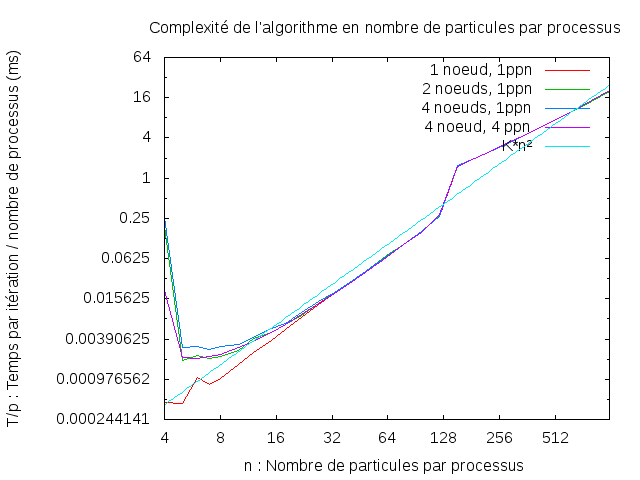
\includegraphics[scale=0.6]{complexity.png}
\caption{Complexité de la simulation}
\label{fig:complexity}
\end{figure}


\subsubsection{Parallélisation}

L'algorithme semble bien se comporter avec la parallélisation puisque les courbes de la figure \ref{fig:complexity} se confondent lorsque le nombre de particules est suffisant. En dessous de 16 particules par processus, la version la plus rapide est celle exécutée sur un seul processus, ensuite les courbes se confondent. Cela n'a rien d'étonnant puisque la taille des calculs croit de manière quadratique alors que celle des communications croit de manière linéaire et qu'en plus les communications sont recouvertes par le calcul.

On remarque aussi que pour n faible, la localité mémoire a son importance : la courbe violette a de meilleure performances bien qu'il y ait plus de processus car ces processus sont sur le même n\oe ud.


\subsection{\'Etude des performances de communications}

Pour vérifier que les calculs recouvrent bien les temps de communication, nous effectuons des calculs à charge égale (même nombre de processus, et de particules par processus) suivant plusieurs configurations possibles : 
\begin{itemize}
\item 1 n\oe ud utilisé avec 6 processus par n\oe ud (ppn) ;
\item 2 n\oe uds utilisés avec 3 ppn ;
\item 3 n\oe uds utilisés avec 2 ppn ;
\item 6 n\oe uds utilisés avec 1 ppn.
\end{itemize}

Si les calculs recouvrent les temps de communications, toutes les configurations devraient donc réaliser les calculs en un même temps, puisque ces configurations répartissent les calculs sur un nombre variable de n\oe uds donc nécessitant des temps de communications non négligeables. C'est ce que nous pouvons constater sur la figure \ref{img:nodes} où le temps de calcul en fonction du nombre de n\oe uds (mais avec un total de processus constant égal à 6) est une droite horizontale. Précisons que ces mesures ont été réalisées pour 10 particules, 10000 itérations et avec un dt automatique.

\begin{figure}
\centering
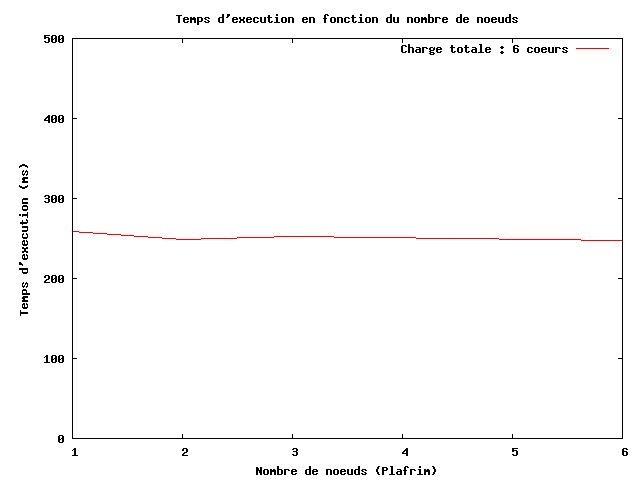
\includegraphics[scale=0.5]{img/graph_nodes.png}
\caption{Temps de calcul en fonction du nombre de n\oe uds impliqués.}
\label{img:nodes}
\end{figure}

\subsection{Comparaison avec un dt automatique}

L'introduction du dt automatique permet une plus grande précision dans les calculs mais nécessite une opération de calcul de racine d'un polynôme du second degré pour chaque particule. Il introduit donc nécessairement un léger surcoût, d'autant qu'il faut ensuite effectuer un \texttt{MPI\_ALLreduce} pour déterminer et communiquer le dt de la prochaine itération à tous les processus.

Cependant la complexité de ce calcul est ainsi linéaire en fonction du nombre de particules (avec toutefois un coefficient élevé), donc asymptotiquement il ne devrait pas induire une trop grande différence avec la version originale (avec un dt constant) puisque la complexité totale du problème est quadratique en le nombre de particules. La figure \ref{img:dt} semble pourant indiquer qu'au contraire l'écart de temps entre les deux versions se creuse, mais il faudrait effectuer ces mesures sur un plus grand nombre de particules pour en être certain.

\begin{figure}
\centering
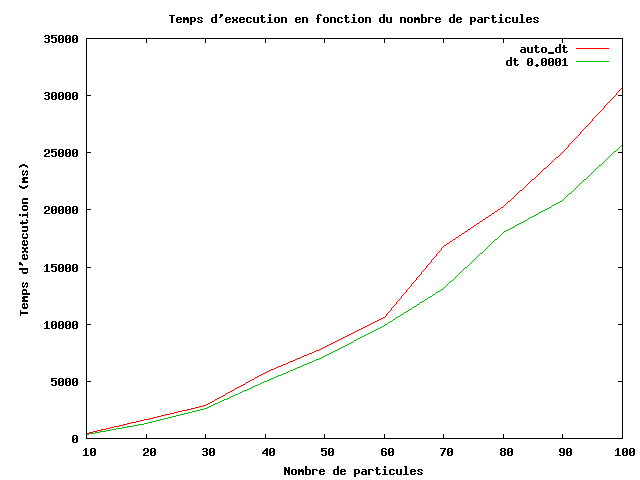
\includegraphics[scale=0.5]{img/graph_auto_dt.png}
\caption{Temps de calcul en fonction du nombre de particules.}
\label{img:dt}
\end{figure}


%\newpage
\section*{Conclusion}
\addcontentsline{toc}{section}{Conclusion}

Nous avons implémenté la simulation du nuage de particules de manière distribuée en utilisant la bibliothèque MPI et analysé les performances de cet algorithme.

Ce qui ressort des benchmarks effectués, est que l'algorithme se parallélise bien car l'accélération obtenue sur une exécution se rapproche fortement du nombre de processeurs. Ce résultat n'est pas étonnant dans la mesure où les calculs (de complexité quadratique) recouvrent rapidement le temps des communications (qui sont de complexité linéaire). 

Différentes techniques ont été mises en \oe uvre pour rendre les communications les plus transparentes possibles, comme la mise en place de communications persistantes et le recouvrement des communications par le calcul. Ces améliorations ont permis d'utiliser les capacités de calcul de manière aussi efficace que l'algorithme séquentiel.

Une autre amélioration à été mise en place, en utilisant un dt variable pour une simulation plus précise. Cette amélioration entraîne cependant un surcoût en temps de calcul.

Des améliorations sont encore possibles, il est notamment possible de diminuer le temps de calcul à chaque itération en optimisant les opérations, mais cela n'entre pas dans le cadre de ce TDP.



\end{document}
